
%(BEGIN_QUESTION)
% Copyright 2012, Tony R. Kuphaldt, released under the Creative Commons Attribution License (v 1.0)
% This means you may do almost anything with this work of mine, so long as you give me proper credit

This production process manufactures {\it ammonium nitrate}, a principal ingredient of synthetic fertilizer, from the chemical combination of nitric acid and ammonia.  The balance of nitric acid to ammonia is critical to controlling the pH of the ammonium nitrate solution exiting the neutralizer.  A combination cascade/feedforward control system exerts control over the nitric acid valve FV-23 while sensing ammonia flow (FT-24) and neutralizer effluent pH (AIT-28a, -28b, and -28c):

$$\includegraphics[width=15.5cm]{i0008rx01.eps}$$

The chemistry of the process is as such: the addition of more nitric acid will drive pH down to lower values.  If ammonia off-gas flow happens to rise, nitric acid flow will also have to rise in order to balance the chemical reactions taking place inside the neutralizer.

\vskip 10pt

Knowing this, explain how this control system works to maintain a stable effluent pH from the neutralizer vessel.  Specifically, identify the primary and secondary cascaded loops, the wild variable and captive variables, and the feedforward dynamic compensation.

\vskip 20pt \vbox{\hrule \hbox{\strut \vrule{} {\bf Suggestions for Socratic discussion} \vrule} \hrule}

\begin{itemize}
\item{} Explain how we could empirically test this system to determine whether the dynamic compensation needs to be {\it lead} or {\it lag}.
\item{} Why are {\it three} different pH transmitters being used to monitor the neutralizer effluent pH?
\end{itemize}

\underbar{file i03394}
%(END_QUESTION)





%(BEGIN_ANSWER)

AIC-28 is the primary (master) pH controller, while FFC-23 is the cascaded secondary (slave) flow controller.  FFC-23 also acts as the summer where the ``wild'' feedforward ammonia vapor flow signal from FT-24 may preemptively call for changes in acid flow rate.  The lead/lag unit, FY-23, of course is the dynamic compensation portion of the feedforward control.
 
%(END_ANSWER)





%(BEGIN_NOTES)


\vskip 20pt \vbox{\hrule \hbox{\strut \vrule{} {\bf Virtual Troubleshooting} \vrule} \hrule}

This question is a good candidate for a ``Virtual Troubleshooting'' exercise.  Presenting the diagram to students, you first imagine in your own mind a particular fault in the system.  Then, you present one or more symptoms of that fault (something noticeable by an operator or other user of the system).  Students then propose various diagnostic tests to perform on this system to identify the nature and location of the fault, as though they were technicians trying to troubleshoot the problem.  Your job is to tell them what the result(s) would be for each of the proposed diagnostic tests, documenting those results where all the students can see.

During and after the exercise, it is good to ask students follow-up questions such as:

\begin{itemize}
\item{} What does the result of the last diagnostic test tell you about the fault?
\item{} Suppose the results of the last diagnostic test were different.  What then would that result tell you about the fault?
\item{} Is the last diagnostic test the best one we could do?
\item{} What would be the ideal order of tests, to diagnose the problem in as few steps as possible?
\end{itemize}


%INDEX% Process: ammonium nitrate production (realistic P&ID shown)

%(END_NOTES)


